\definecolor{codegreen}{rgb}{0,0.6,0}
\definecolor{codegray}{rgb}{0.5,0.5,0.5}
\definecolor{codepurple}{rgb}{0.58,0,0.82}
\definecolor{backcolour}{rgb}{0.95,0.95,0.92}

\lstdefinelanguage{Godot}{
	keywords={class_name, func, for, return, in range, is, var, not, continue, or},
	morecomment=[l]{#}
}

\lstdefinelanguage{dict}{
	keywords={class_name, func, for, return, in range, is, var, not, continue},
}

\lstdefinestyle{mystyle}{
    backgroundcolor=\color{backcolour},   
    commentstyle=\color{codegreen},
    keywordstyle=\color{magenta},
    numberstyle=\tiny\color{codegray},
    stringstyle=\color{codepurple},
    basicstyle=\ttfamily\footnotesize,
    breakatwhitespace=false,         
    breaklines=true,                 
    captionpos=b,                    
    keepspaces=true,                 
    numbers=left,                    
    numbersep=5pt,                  
    showspaces=false,                
    showstringspaces=false,
    showtabs=false,                  
    tabsize=2
}

\lstset{style=mystyle}



\chapter{GOAP Umsetzung in Godot}

Die praktische Umsetzung des GOAP Systems wird nun in diesem Kapitel beschrieben. Die Umsetzung passiert auf Basis der Publikation von Jeff Orkin \autocite{}. Die Implementierung geschieht unter der Godot Engine 4.3. Das Kapitel wird zuerst die grundlegende Architektur von GOAP anhand eines Agenten beschreiben.[Kapitel weiter erläutern]



\section{GOAP Architektur}

Die folgende Abbildung soll die grundlegende Architektur von GOAP darstellen. Die Architektur wurde in Godot 4.3 umgesetzt und dient als Basis für die Bewertung in den weiteren Kapiteln. Die Darstellung wird anhand eines Klassendiagramms in UML-Notation umgesetzt.

\begin{figure}[h]
  \centering
  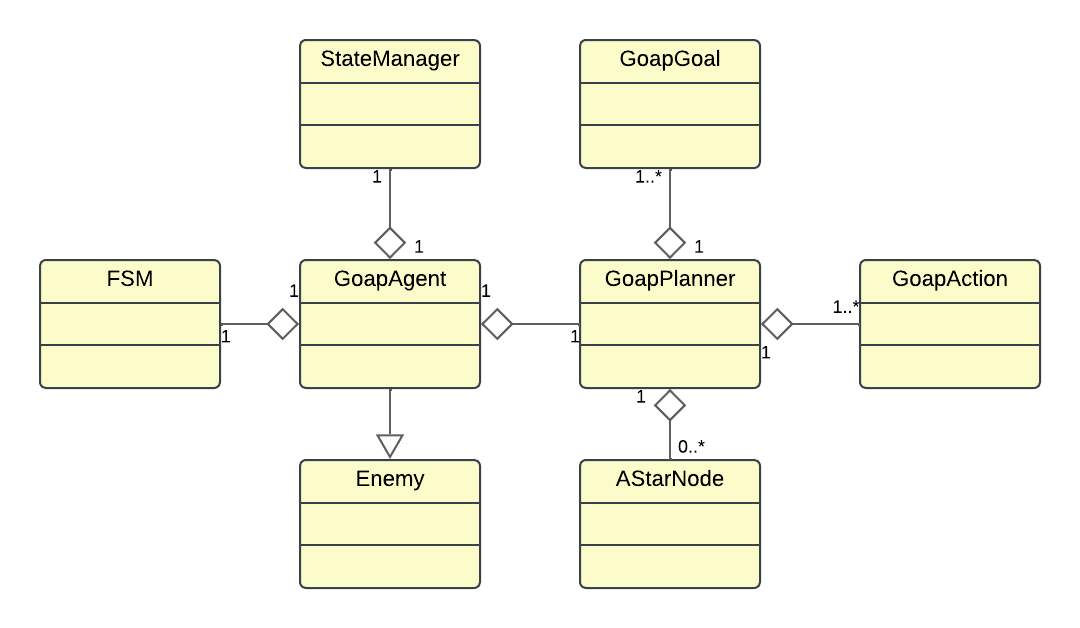
\includegraphics[width=16cm]{GOAP_2/GOAP_UML}
	\captionsetup{justification=justified, format=plain}
  \caption{GOAP Architektur}
  \label{GOAP Architektur eines Agenten}
\end{figure}

Aus dem GOAP-Kapitel geht hervor, dass ein GOAP-System aus einem Planner, Zielen, Aktionen und einer FSM (Finite State Machine) besteht. Diese Komponenten erfüllen ihre jeweiligen Aufgaben, wie im Grundlagenkapitel zu GOAP beschrieben.

Der GoapAgent bildet dabei die Hauptklasse und fungiert als Schnittstelle zur restlichen Spielwelt. Die Spielwelt kann dem GoapAgent Informationen wie die Position des Spielers oder bestimmte Koordinaten innerhalb der Spielwelt übermitteln. Dabei erbt der GoapAgent von der Klasse Npc. Die Klasse Npc stellt Komponenten bereit, die es dem GoapAgent ermöglichen, mit der Spielwelt zu interagieren.

Der StateManager verwaltet die Zustände des NPC. Diese Zustände können über die Komponenten der Oberklasse Npc oder durch nichtdeterministische Umstände der Spielwelt verändert werden. Die Zustandsabfragen für die Auswahl des Zieles und Aktionen erfolgen über diese Klasse.

Zur Generierung von Sequenzen und Festlegung des Zieles benutzt der GoapAgent die Klasse GoapPlanner. Der GoapPlanner besitzt dabei Objekte der Klasse GoapGoal. Aus diesen Objekten wählt der GoapPlanner einen Zielzustand aus, für den eine Aktionssequenz gesucht wird. Der GoapPlanner sucht seine Sequenz mithilfe des A* Suchalgorithmus. Die Klasse AStarNode wird zur Generierung von Knoten für den A* Suchalgorithmus benötigt. Ein AStarNode setzt dabei die Eigenschaften eines Suchbaum-Knoten um.

Die Klasse GoapAction stellt die Basisklasse für Aktionen dar. Eine Aktion repräsentiert dabei eine Kante im Suchbaum und wird entsprechend als solche im AStarNode-Objekt gespeichert.

Es wird keine Finite State Machine (FSM) in der Architektur umgesetzt, da die Implementierung keine Animationen umfasst. Stattdessen geschieht die Ausführung der Aktionen direkt aus der Klasse GoapAgent. Sollten Animationen vorhanden sein, können diese auch über die Klasse GoapAction ausgeführt werden. Es besteht keine zwingende Notwendigkeit, eine FSM innerhalb von GOAP umzusetzen. Ein Konzept für die Implementierung einer FSM wäre es, diese an den GoapAgent oder GoapPlanner zu koppeln und die Aktionssequenz von dort aus auszuführen. Die Aktionen würden dann auch die Zustandswechsel für die FSM durchführen.


\subsection{GoapAgent}

% Zusammenfassung
Folgende Abbildung stellt die Klasse GoapAgent dar. Die Darstellung wird anhand eines Klassendiagramms in UML-Notation umgesetzt. Der GoapAgent speichert folgende Klassenvariablen: goap\_planner, action\_sequence und den current\_step. Bei den Methoden handelt es sich um: update und follow\_sequence. 

% Klasse Npc
Unter anderem erbt die Klasse Komponenten der Klasse Npc. Die Komponenten dienen dem NPC zur Wahrnehmung und Manipulation der Videospielumgebung. Ein Beispiel einer solchen Komponente ist die vision\_component, welche über die update Methode aufgerufen, wird um den Spieler zu erfassen.


\subsubsection{Klassenattribute}

Der goap\_planner ist eine Referenz auf die Klasse GoapPlanner, welche das Ziel und die action\_sequence des GoapAgent bestimmt. Das Array action\_sequence speichert Objekte vom Typ der Klasse GoapAction. Sie stellt die ermittelte Aktionssequenz durch den A* Algorithmus dar. Die Integer-Klassenvaraible current\_step handelt als Indexzeiger, welcher auf die aktuell auszuführende Aktion des action\_sequence verweist.

% Goap Agent
\begin{figure}[h]
  \centering
  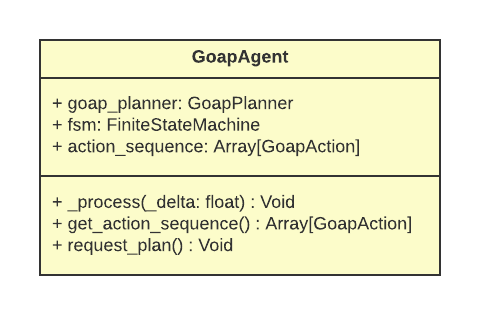
\includegraphics[width=10cm]{GOAP_2/GoapAgent_UML}
	\captionsetup{justification=justified, format=plain}
  \caption{GOAP Agent}
  \label{GOAP Agent}
\end{figure}


\subsubsection{Methoden}

Die Methode update wird durch eine \_process Funktion jedes \textit{Frame} aufgerufen, um kontinuierliche Logik wie Bewegungen oder Raycasting des GoapAgent zu verarbeiten. Die \_process Funktion wird von Godot 4.3 bereitgestellt. Sie befindet sich in der Komponente, welche das Objekt GoapAgent instanziiert. Die update Methode ruft Methoden der Klassen und Komponenten innerhalb des NPC auf. Der Parameter delta repräsentiert die Zeit seit dem letzten Frame und könnte an andere Methoden übergeben werden.

% update Methode
\lstinputlisting[firstline=2, language=Godot, linerange={12,14-17,19}, caption={update Methode des GoapAgent}, label=lst:caption]{code/goap_enemy.gd}

In der update Methode wird eine Abfrage gestellt, ob der goap\_planner eine neue action\_sequence generiert hat. Wurde eine neue action\_sequence generiert, so wird die Objektvariable current\_step auf $0$ zurückgesetzt und die neue action\_sequence aus dem goap\_planner abgerufen. Die action\_sequence wird dann durch die Methode follow\_sequence ausgeführt.

% follow_sequence Methode
Über die Methode follow\_sequence geschieht die Ausführung der Aktionen aus der action\_sequence. Sollte action\_sequence leer sein, bereits ausgeführt worden oder ungültig sein, so wird eine neue action\_sequence von dem goap\_planner gefordert. Ansonsten wird mithilfe des current\_step Index die jeweilige Aktion über ihre GoapAction.update Methode ausgeführt. Bei erfolgreicher Ausführung der Aktion wird der current\_step inkrementiert, um auf die nächste Aktion der action\_seqeunce zugreifen zu können.

\lstinputlisting[firstline=2, language=Godot, linerange={21-28}, caption={follow\_sequence Methode des GoapAgent}, label=lst:caption]{code/goap_enemy.gd}



\subsection{GoapPlanner}

% Zusammenfassung
Folgende Abbildung zeigt die Struktur des GoapPlanner, anhand eines Klassendiagramms in UML-Notation. Die Klassenvariablen und Methoden können in der folgenden Abbildung entnommen werden.

\begin{figure}[h]
  \centering
  \includegraphics[width=10cm]{GOAP_2/GoapPlanner_UML}
	\captionsetup{justification=justified, format=plain}
  \caption{GoapPlanner}
  \label{GoapPlanner}
\end{figure}


\subsubsection{Klassenattribute}

Der GoapPlanner arbeitet mit Zielen und Aktionen, welche durch die Arrays actions und goals gegeben werden. Über current\_goal wird das Ziel gespeichert, zu dem eine action\_sequence gesucht wird. Die action\_sequence ist die generierte Aktionssequenz durch den GoapPlanner und wird in einem Array mit GoapAction als Elementtyp gespeichert. 

Das current\_state Dictionary speichert den derzeitigen Zustand des NPC. Die Initialisierung des current\_state findet über den state\_manager Parameter statt, welcher über die update Methode übergeben wird.

Das create\_sequence Attribut informiert den GoapPlanner darüber, ob eine neue action\_sequence generiert werden soll.

% effect_action_dict
Das effect\_action\_dict Dictionary speichert alle Zustände als \textit{key} und die Aktionen, welche den Zustand beeinflussen können als \textit{values}. So erhält man eine schnellere Zugriffszeit, als wenn man jeden Effekt einer Aktion im Array mit dem benötigten Zustand vergleicht.

\begin{lstlisting}[language=dict, caption={effect\_action\_dict aus der Implementierung}]
effect_action_dict = {
    "player_eliminated": [
        RangedAttackFromCover:<Node#82829117475>,
        MeleeAttack:<Node#82845894692>,
        RangedAttack:<Node#82812340258>
    ],
    "player_block_visited": [
        GoToNode:<Node#82862671909>
    ],
    "at_patrol_node": [
        GoToNode:<Node#82862671909>
    ],
    "at_cover_node": [
        GoToNode:<Node#82862671909>
    ],
    "bullets": [
        Reload:<Node#82879449126>
    ]
}
\end{lstlisting}


\subsubsection{Methoden}

% update
Die GoapPlanner Methode update wird über die update Methode des GoapAgent aufgerufen. Hierbei werden Methoden und Abfragen durchgeführt, welche die current\_goal und die dazugehörige action\_sequence bestimmen. 

Für die Bestimmung des current\_goal ist die Methode get\_best\_goal verantwortlich. Ändert sich das Ziel während der Laufzeit oder wird über create\_sequence eine action\_sequence angefragt, so soll eine neue action\_sequence generiert werden. Die Suche geschieht über die Methode create\_new\_sequence. 

\lstinputlisting[firstline=2, language=Godot, linerange={16-22}, caption={update Methode des GoapPlanner}, label=lst:caption]{code/goap_a_star_planner.gd}

% create_new_sequence Methode
Die Methode create\_new\_sequence leitet die Generierung einer action\_sequence ein. Dafür muss ein Wurzelknoten des Typen AStarNode erstellt werden, welcher dem a\_star\_algorithm übergeben wird. Für den Wurzelknoten wird ein Dictionary über die Methode create\_current\_state\_of\_goals instanziiert, in dem die Werte der Zielzustände des current\_goal basierend auf den Werten des current\_state des Agenten überschrieben werden. Das Dictionary wird als Zustand des Wurzelknoten dienen, mit dem die a\_star\_algorithm Methode nach der Aktionssequenz sucht. Die Funktionsweise der a\_star\_algorithm Methode wird im folgenden Quellcode kommentiert. Sie sucht nach den Regeln, welche im Kapitel A$^*$ Algorithmus beschrieben werden.

\lstinputlisting[firstline=2, language=Godot, linerange={42-59}, caption={a\_star\_algorithm Methode des GoapPlanner}, label=lst:caption]{code/goap_a_star_planner.gd}

% PriorityQueue
Die open\_list wird über eine PriorityQueue realisiert. Man beachte, dass Godot 4.3 keine PriorityQueue besitzt und man diese selbst implementieren müsste. Eine PriorityQueue speichert Knoten, sortierter nach ihren $f(n)$ Kosten, sodass Knoten mit den niedrigsten Kosten bevorzugt abgerufen werden. Die Umsetzung befindet sich im Anhang...

% expand_node Methode
Die expand\_node Methode fügt Kindknoten child\_node des expandierten Knoten expanded\_node in die open\_list, welche vorher von A$^*$ gewählt wurde. Es folgt die Instanziierung der Kosten $g(n)$, $h(n)$ und $f(n)$ des child\_node. Abschließend wird der child\_node in die \textit{open\_list} hinzugefügt.

\lstinputlisting[firstline=2, language=Godot, linerange={61-79}, caption={expand\_node Methode des GoapPlanner}, label=lst:caption]{code/goap_a_star_planner.gd}

% get_child_nodes Methode
Die get\_child\_nodes Methode sucht nach Kanten (Aktionen) welche die benötigten Zustände des Knoten erfüllen können. Dabei werden die benötigten Zustände mit den Zuständen der effect\_action\_dict verglichen.

Wird eine Aktion gefunden, welche den Zustand erfüllt, so wird untersucht ob der Effekt, der Aktion den Zustand umsetzen kann. Erfüllt der Effekt den gewünschten Zustand, so wird ein Kindknoten erstellt. Dieser Kindknoten speichert die Kante (Aktion) die zu dem Knoten geführt hat, sowie den Effekt auf den current\_state. Die restlichen Inhalte des Knoten werden in der zuvor beschriebenen expand\_node Methode instanziiert.

\lstinputlisting[firstline=2, language=Godot, linerange={}, caption={get\_child\_nodes Methode des GoapPlanner}, label=lst:caption]{code/goap_a_star_planner.gd}

% create_path Methode
Wenn a\_star\_algorithm einen expand\_node expandiert und dieser keine zu erfüllenden Zustände mehr besitzt, wurde der optimale Pfad gefunden. Um nun die korrekte action\_sequence zu erhalten, müssen die Aktionen vom expand\_node rekursiv zum Wurzelknoten zurückverfolgt werden. Dies wird mithilfe einer \textit{create\_path} Methode durchgeführt.


\subsection{AStarNode}

Der AStarNode hat die Funktionsweise eines Knoten in einem Suchbaum. Sie werden über die get\_child\_node Methode instanziiert. Folgende Abbildung zeigt die Struktur der Klasse AStarNode in der UML-Notation.

\begin{figure}[h]
  \centering
  \includegraphics[width=10cm]{GOAP_2/AStarNode_UML}
	\captionsetup{justification=justified, format=plain}
  \caption{AStarNode}
  \label{AStarNode}
\end{figure}


\subsubsection{Klassenattribute}

Ein AStarNode speichert die Informationen des Suchproblems. Darunter die bis dahin erfüllten Zustände des Elternknoten parent\_node im Attribut current\_state\_of\_goals, sowie alle Zielzustände die bis zu dem Knoten benötigt wurden im Attribut goal\_state. Über das Klassenattribut parent\_node kann die create\_path Methode des GoapPlanner rekursiv auf die Aktionen action des Typs GoapAction zurückschließen. Die Kosten $f(n)$ werden unter f\_cost und $g(n)$ -Kosten unter g\_cost gespeichert.


\subsubsection{Methoden}

Durch den Godot Konstruktor \_init wird ein AStarNode mit seinen Attributen instanziiert. Die Berechnung der Kosten passiert durch die GoapPlanner Methode expand\_node. Dort werden über die setter- Methoden des AStarNode set\_g\_cost und set\_f\_cost initialisiert. Über die Methode get\_unsatasfied\_states werden alle Zustände zurückgegeben, welche noch nicht erreicht wurden. Die Größe des Arrays welches von get\_unsatasfied\_states gegeben wird repräsentiert die heuristischen Kosten $f(n)$ der Aktion. Die Heuristik Kosten werden ebenfalls in der expand\_node Methode des GoapPlanner berechnet und initialisiert.

Wird eine action gewählt, so wird ein AStarNode mit den dazugehörigen Zuständen current\_state\_of\_goals und goal\_states generiert werden. Die Generierung des neuen AStarNode geschieht über die apply\_action\_to\_state Methode. Die Methode wird vom GoapPlanner durch die Methode get\_child\_nodes auf dem expanded\_node aufgerufen. Dabei wird die action und der current\_state als Parameter übergeben. Basierend auf den Parameter initialisiert die Methode, die Attribute goal\_states und current\_state\_of\_goals für den neuen Knoten. Außerdem initialisiert sie den zu expandierten Knoten als parent\_node sowie die Aktion als action.

Die Prüfung ob die Zustände eines expanded\_node erfüllt wurden, wird durch is\_satasfied geprüft. Dazu schaut die Methode ob das Array welches über die Methode get\_unsatasfied\_states zurückgegeben wird leer ist. Sollte das Array leer sein, so gibt es keine zu erfüllenden Zustände und der AStarNode ist der Zielknoten.


\subsection{GoapGoal}

Ein GoapGoal repräsentiert ein Ziel. Der GoapPlanner bewertet die verfügbaren Ziele, vergleicht sie miteinander und wählt eines aus, basierend auf deren Gültigkeit und Priorität. Der Zielzustand des jeweiligen GoapGoal wird als Ausgangszustand für Suche genutzt. Die Klasse GoapGoal wird in der folgenden Abbildung mittels UML-Notation dargestellt.

\begin{figure}[h]
  \centering
  \includegraphics[width=10cm]{GOAP_2/GoapGoal_UML}
	\captionsetup{justification=justified, format=plain}
  \caption{GoapGoal}
  \label{GoapGoal}
\end{figure}

Die Priorität und Gültigkeit wird aus dem Klassenattribut state\_manager abgeleitet. Die get\_best\_goal des GoapPlanner benötigt die Gültigkeit und Priorität, um in folge dessen das Ziel auszuwählen. Die Abfragen geschehen durch die Methoden get\_priority und is\_valid. Ein Ziel wird erst dann berücksichtigt, wenn es durch die Methode is\_valid als gültig bestätigt wurde. Anschließend kann dessen Priorität mithilfe von get\_priority ermittelt werden. 

Über die Methode get\_desired\_state werden die Zielzustände aufgerufen, welche der GoapPlanner zur Suche der action\_sequenz benötigt. 

Die Methode get\_goal\_name gibt den Klassennamen des GoapGoal zurück, welche von Debug Methoden genutzt werden kann.


%FORTSETZUNG
\subsection{GoapAction}

Ein Aktion des Typs GoapAction, repräsentieren die Kanten eines Suchbaums. Sie besitzen Daten zur Generierung eines neuen Knoten. Folgende Abbildung stellt die GoapAction Klasse nach UML-Notation dar.

\begin{figure}[h]
  \centering
  \includegraphics[width=10cm]{GOAP_2/GoapAction_UML}
	\captionsetup{justification=justified, format=plain}
  \caption{GoapAction}
  \label{GoapAction}
\end{figure}

Mit Hilfe der Klassenattribute character\_body und state\_manager werden die Kosten $g(n)$ und die Gültigkeit der Aktion gelesen. Die Kosten $g(n)$ werden dabei über die get\_cost Methode berechnet.

Die Gültigkeit einer Aktion soll die Durchführbarkeit wiedergeben. Der GoapPlanner wählt nur Aktionen aus, welche im derzeitigen Zustand des NPC durchführbar sind. Die Gültigkeit der Aktionen wird auch vor der Ausführung der update Methode jeweiligen Aktion durch den GoapAgent geprüft, da die Aktion zu einer Zeit ausgeführt werden kann in der sich der Zustand des NPC wieder ändern kann und somit auch die Gültigkeit. Für die Rückgabe der Gültigkeit ist die is\_valid Methode zuständig.

Eine get\_preconditions Methode gibt die vorausgesetzten Zustände zurück, welche von anderen Aktionen erfüllt werden müssten. Ob eine Aktion einen Zustand erfüllen kann, hängt von der get\_effects Methode ab, welche ein \textit{Dictionary} mit dem Zustand und dessen Wert zurückgibt. Stimmt der Wert des Zustands mit dem Zielzustand überein, dann erfüllt die Aktion den Zustand.

Die update Methode leitet die eigentliche Ausführung der Aktion ein und wird über den GoapAgent gestartet. Die Hoffnung dabei ist, dass die Aktion den erwünschten Wert des Effekts umsetzt. Aufgrund der nicht-deterministischen Natur der Spielwelt kann es jedoch vorkommen, dass der angestrebte Effekt nicht erreicht wird. Wird der Effekt nicht erreicht, so wird eine neue Sequenz angefordert oder das Ziel ändert sich bis dahin. Die Ausführung der Aktion wird dabei über Komponenten der Klasse Npc umgesetzt. Die Methode get\_action\_name gibt den Klassennamen der GoapAction zurück.

%\lstinputlisting[firstline=2, language=Godot, linerange={}, caption={Die Aktion RangedAttack erbt von GoapAction}, label=lst:caption]{code/goap_ranged_attack.gd}

